
\begin{center}

  \textsf{\MakeUppercase{Wilkinson (2005)}}

\smallskip

\textsf{\MakeUppercase{Chapter 13}}

\smallskip

\textsf{\MakeUppercase{Notes by Mick McQuaid}}

\end{center}


\hypertarget{space}{%
\section{Space}\label{space}}

Wilkinson defines a graphics frame as a set of tuples ranging over all
possible values in the domain of a \(p\)-dimensional varset. Already we
are defining terms using other terms previously defined in the book, and
defined in a casual way. A tuple, \((a,b)\) is a pair and an \(n\)-tuple
is a set, \((a_1, a_2, \ldots, a_n)\).

But a pair of what? A set of what? What can you depict in a graphic? It
seems that only correspondences can be depicted. There can't be a single
object; there must be at least two. Is that true?

Wilkinson defines \emph{graph} in two different ways: (1) a subset of
the tuples in a graphics frame and (2) as a set of vertices and edges
(which is the graph-theoretic definition of a graph). This can be
confusing as the chapter develops, since he explores different ways to
think about space, including the graph-theoretic approach.

Wilkinson defines a graphic as the perceptual realization of a graph
(first sense) and claims we use two spaces to make a graphic: the
underlying space with a mathematical definition and a display space
which is always \(2D\) or \(3D\) Euclidean space.

He gives an example of a graphical depiction of beadlet anemones on a
rock, showing a photograph of them and two minimum spanning trees
describing them. He actually defines minimum spanning trees later in the
chapter but suffice it for now to say that more than one is possible and
that one might be preferred over another for some purposes. By the way,
Wikipedia gives what I consider a better definition of a minimum
spanning tree as a subset of the edges of a connected, edge-weighted
undirected graph that connects all the vertices together, without any
cycles and with the minimum possible total edge weight.

In Wilkinson's example, the two minimum spanning trees arise from two
different sets of information about the beadlet anemones. One is the
\((x,y)\) coordinates of the anemones on the rock (as if it were a
plane) while the other is a list of anemone name pairs and weights for
the implied edges between them. In the first case, we generate the
weights from the \((x,y)\) coordinates and in the other case, the
weights are given. In both cases, the output is a display of a tree in
two-dimensional space on the page of the book.

The two trees look different from each other but we have no way of
knowing whether the difference matters unless we know something about
the underlying space which, in this case, means knowing the underlying
given data.

Thus concludes Wilkinson's introduction to space. Next he considers the
mathematical concept of space, the psychological concept of space, and
the graph-theoretic concept of space.

\hypertarget{mathematical-space}{%
\section{13.1 Mathematical space}\label{mathematical-space}}

The next section of the book is devoted to a description of popular
mathematical spaces for graphics. All of these are topological and are
subsets of topological spaces. These spaces obey some mathematical
axioms which are listed and some of them are metric, defined by another
set of axioms.

Some of these spaces are connected in the sense that they can't be
partitioned and some are totally disconnected in that each point is in
its own space as is a graphic of entirely categorical variables.
Continuous variables are embedded in a connected space. If you have
continuous and categorical variables in the same graphics frame, you
have a set of connected spaces, which lead to empty regions in graphics.
The result is the opportunity to use the empty space to encode
additional sources of variation using aesthetics (things we can see,
such as color and position).

Metric spaces can be problematic. We can't encode information that
violates the three axioms I mentioned earlier, identity, symmetry, and
the triangle inequality in a metric space.

\hypertarget{maps}{%
\subsection{13.1.4 Maps}\label{maps}}

Wilkinson then defines maps (not the geographic kind, the topological
kind) that can be injective, surjective, or bijective. The map,
\(f:X\rightarrow Y\) is injective if no element in \(Y\) has more than
one element of \(X\) mapped to it. It is surjective if every element in
\(Y\) has at least one element of \(X\) mapped to it, and it is
bijective if it is both injective and surjective. Why you need to know
this is unclear at the moment. It leads into the following definition,
though, and may be helpful there.

\hypertarget{embeddings}{%
\subsection{13.1.5 Embeddings}\label{embeddings}}

A map \(f:S\rightarrow P\) from one topological space to another is an
embedding if \(S\) and its image \(f(S)\) in \(P\) are homeomorphic. A
homeomorphism is a continuous one-to-one function whose inverse is also
continuous. Continuous means that points that are arbitrarily close in
\(S\) are also arbitrarily close in \(P\).

It would be wonderful if the relationship between our mathematical space
and physical space were an embedding, but it often isn't and this
explains, in a mathematical sense, why many visualizations can't work or
are intrinsically hard to comprehend. There is a famous case where
Milton Friedman, the economist, used dots that were too large on a
graphic and misinterpreted some major economic phenomenon as a result:
two objects that were arbitrarily close in \(P\) were actually far apart
in \(S\). On the other hand, there are plenty of cases, like planar
geographic maps, that are not embeddings but are useful representations.

\hypertarget{multidimensional-scaling}{%
\subsection{13.1.6 Multidimensional
scaling}\label{multidimensional-scaling}}

The opposite of representing the relationship between points in a known
space is to create space based on known relationships. This is called
multidimensional scaling and begins with dissimilarities between points.

\hypertarget{geodesics}{%
\subsection{13.1.7 Geodesics}\label{geodesics}}

Geodesics are locally length-minimizing paths. In Euclidean \(2D\) space
they are lines, while on a sphere, they are arcs of great circles.
Geodesics need algorithms for determining shortest paths, so they depend
on the definition of a spatial metric.

\hypertarget{dimensions}{%
\subsection{13.1.8 Dimensions}\label{dimensions}}

How do you define the word dimension? A naive definition is the number
of coordinates needed to represent an instance of an object in a
Euclidean space. For example, a point is one, a circle is two, and a
sphere is three.

On the other hand, you only need two coordinates to locate a point on a
sphere. This exemplifies a more sophisticated definition as the number
of coordinates needed to specify a point on an object.

People assign many different meanings to the word dimension. For
example, the term \(2\frac{1}{2}D\) is used by computer scientists,
vision scientists, and geographers to refer to \(2D\) displays with the
half dimension depicting metadata that lets us construct a \(3D\) scene
in our minds from the \(2D\) representation. As another example,
dotplots are really one-dimensional but take up two dimensions so that
there is someplace to put the dots.

\hypertarget{connected-spaces}{%
\subsection{13.1.9 Connected spaces}\label{connected-spaces}}

These are mostly metric spaces. The most common form of metric spaces is
defined by Minkowski distance between two points \(x_j\) and \(x_k\) as
follows.

\[
d(x_j,x_k)=\left(\sum_{i=1}^n \vert x_{ij}-x_{ik}\vert^p\right)^{1/p}
\]

This is a general formula that can be specified for different numbers of
dimensions, \(p\). If \(p=2\) this is Euclidean distance. If \(p=1\)
this is city-block or Manhattan distance. Different distance metrics
distort visualizations in different, sometimes surprising ways.

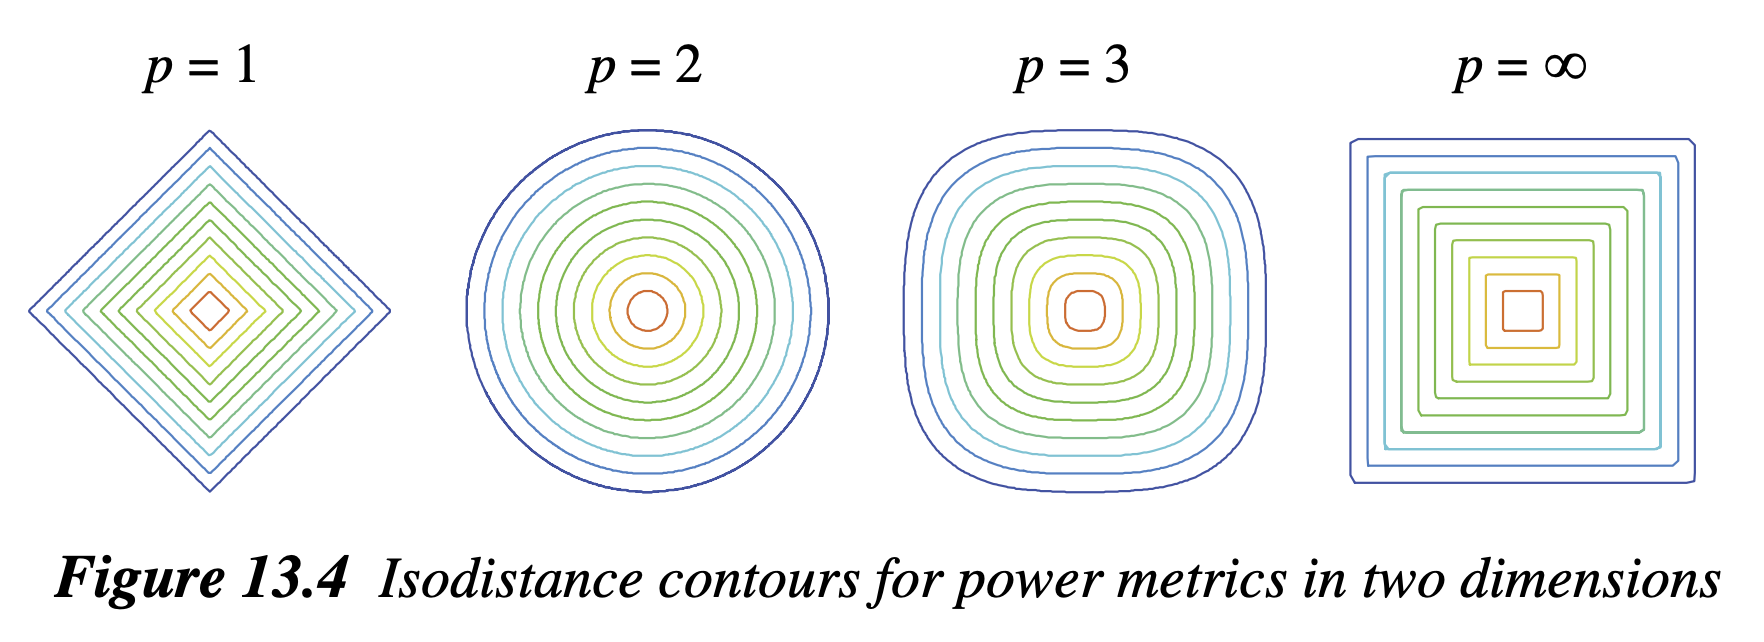
\includegraphics[width=4in,height=1.5in]{fiIsodistances.png}

The textbook's Figure 13.4 shows isodistance contours for different
dimensions, using the above formula. If \(p<1\) as below, the contours
take on an emaciated look that diminishes until we get to the circle at
\(p=2\). Beyond \(p=2\), the contours become more and more square until
at \(p=\infty\) they are perfectly square.

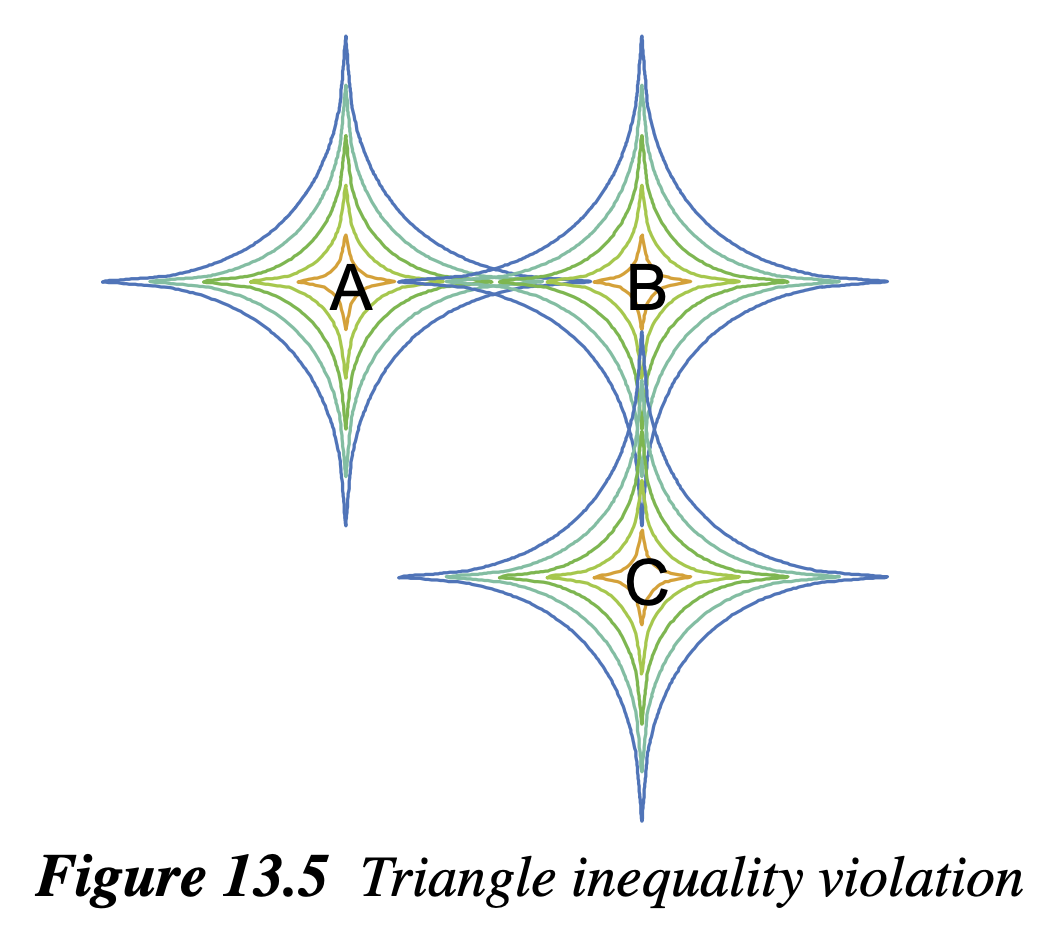
\includegraphics[width=2.00in,height=2in]{fiTriangIneq.png}

The textbook's Figure 13.5 shows a violation of the triangle inequality
because the distance from A to C is so much greater (given the contours)
than the sum of the distances AB and BC.

Wilkinson next describes assymetric distance maps, where the distance
from point \(x_j\) to \(x_k\) is not the same as the distance from
\(x_k\) to \(x_j\). Distance is directional and can be shown by
isocontour lines with an asymmetrical shape.

Visualizations often depict shortest paths. Of particular interest is
the shortest path in \(3D\) space, with the associated concept of the
gradient. The gradient here can be thought of as the path a ball would
take rolling down a smooth hill.

\hypertarget{fractals}{%
\subsection{13.1.10 Fractals}\label{fractals}}

Wilkinson discusses fractals, which are shapes where each part is
similar to the whole and where the shape's Hausdorff dimension differs
from its topological dimension. The definition of the Hausdorff
dimension is beyond the scope of the book and is used only to justify
the exclusion of fractals from the set of objects characterized by their
topological dimensions.

In classifying fractals outside the realm of objects characterized by
topological dimensions, Wilkinson seems to relegate them to a niche in
visualization. However, he offers one example of a fractal being used to
visualize another phenomenon (in other words, not just as a picture of a
fractal for the sake of the fractal's beauty). This comes later in the
chapter and is an example of gene sequences encoded as a fractal that
can be observed from many angles.

\hypertarget{graph-theoretic-space}{%
\subsection{13.1.12 Graph-theoretic space}\label{graph-theoretic-space}}

This subsection covers some basic definitions of graph theory which are
necessary to visualize social networks (or other networks, it's just
that social networks are currently popular in the visualization world).
I'm not going to repeat these definitions here and they are incomplete
in any case.

\hypertarget{psychological-space}{%
\section{13.2 Psychological space}\label{psychological-space}}

This section begins with the observation that Pavlov believed that the
brain is an associative network in which evocation of a response to a
stimulus is likely to activate spatially associated cortical events.
This idea, called spreading activation, remains popular over a hundred
years later.

Wilkinson goes on to mention theories of perception and notes that most
of them postulate at least two stages of processing: (1) pre-attentive
stages, where we perceive a stimulus without effort, and (2) higher
cognitive stages, in which we analyze aspects of the stimulus to make
judgments. So the rest of this section discusses these two stages.

\hypertarget{spatial-models-of-pre-attentive-cognitive-processes}{%
\subsection{13.2.1 Spatial models of pre-attentive cognitive
processes}\label{spatial-models-of-pre-attentive-cognitive-processes}}

Pre-attentive visual and auditory processes appear to be spatial, but
complicated. Some research has suggested that perceived color space is
metric. This is exemplified by the textbook's Figure 13.14, showing on
the left a diagram of chromaticity used for color calibration, and on
the right a picture of judgments about color similarity configured using
multidimensional scaling.

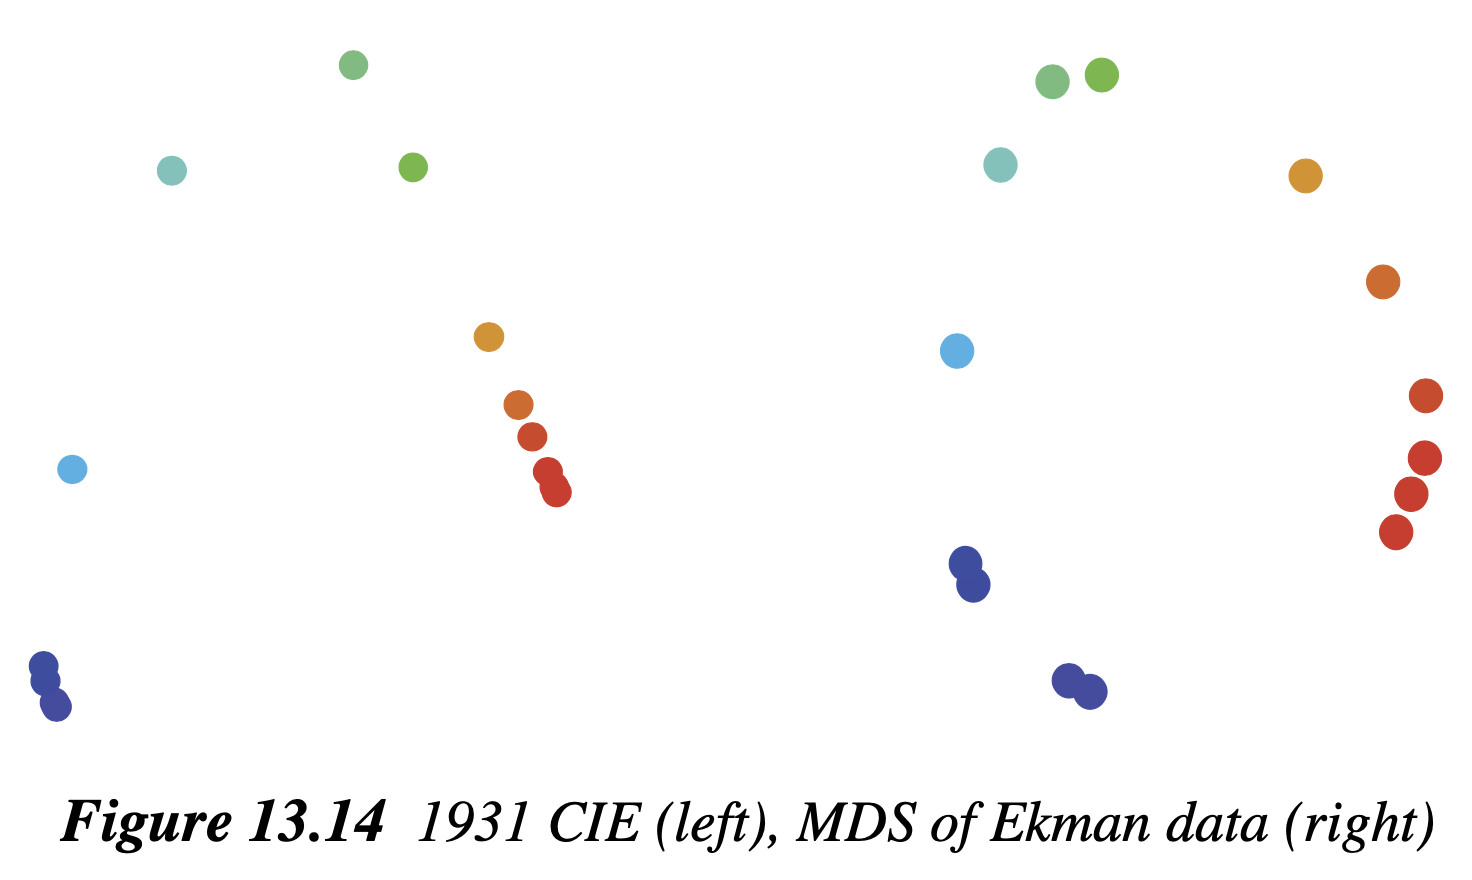
\includegraphics{fiCIEvsMDS.png}

The important point about Figure 13.14 is how similar the two pictures
are, suggesting that pre-attentive human perceptions of color are
metric. Wilkinson gives another example, this time of the pre-attentive
perception of form.

\hypertarget{spatial-models-of-cognitive-processes}{%
\subsection{13.2.2 Spatial models of cognitive
processes}\label{spatial-models-of-cognitive-processes}}

Judgment is a different matter. There is plenty of evidence that human
judgment is not metric, much of it supplied by Amos Tversky and Daniel
Kahnemann in the 1970s and 80s and later summarized for the layperson in
the popular (and controversial!) book \emph{Thinking Fast and Slow}
(2011).

Tversky and Kahnemann show that we can not assume that people will judge
quantities and relationships the same way after a glance and after
lengthy consideration.

A related issue is that we must consider biases introduced by cognitive
processes when people judge spatial material. Another Tversky, Barbara
Tversky, showed that adding a political boundary on a map changes the
judgment of distances between towns in that map.

\hypertarget{spatial-cognition}{%
\subsection{13.2.3 Spatial cognition}\label{spatial-cognition}}

We need to also consider how we perceive and think about space itself.
Evidence shows that the perceptual world is not Euclidean. In the
outdoors we seem to see a flattened spherical world, with the sky
perceived as closer at the zenith than at the horizon. The moon
illusion, in which the moon is perceived as larger at the horizon than
overhead has been cited as evidence of this perception. Indoors, spatial
perception is influenced by the structure of the room. A famous artifact
called the Ames room, with distorted walls, plays tricks on our
perception. (I vividly remember visiting an Ames room in an amusement
park as a child and being so disoriented that I staggered around!) The
Ames room illusion makes people look gigantic or tiny depending on where
they stand, and makes balls appear to roll uphill. I'm attaching a
picture of one uploaded by the UK Royal Institution.

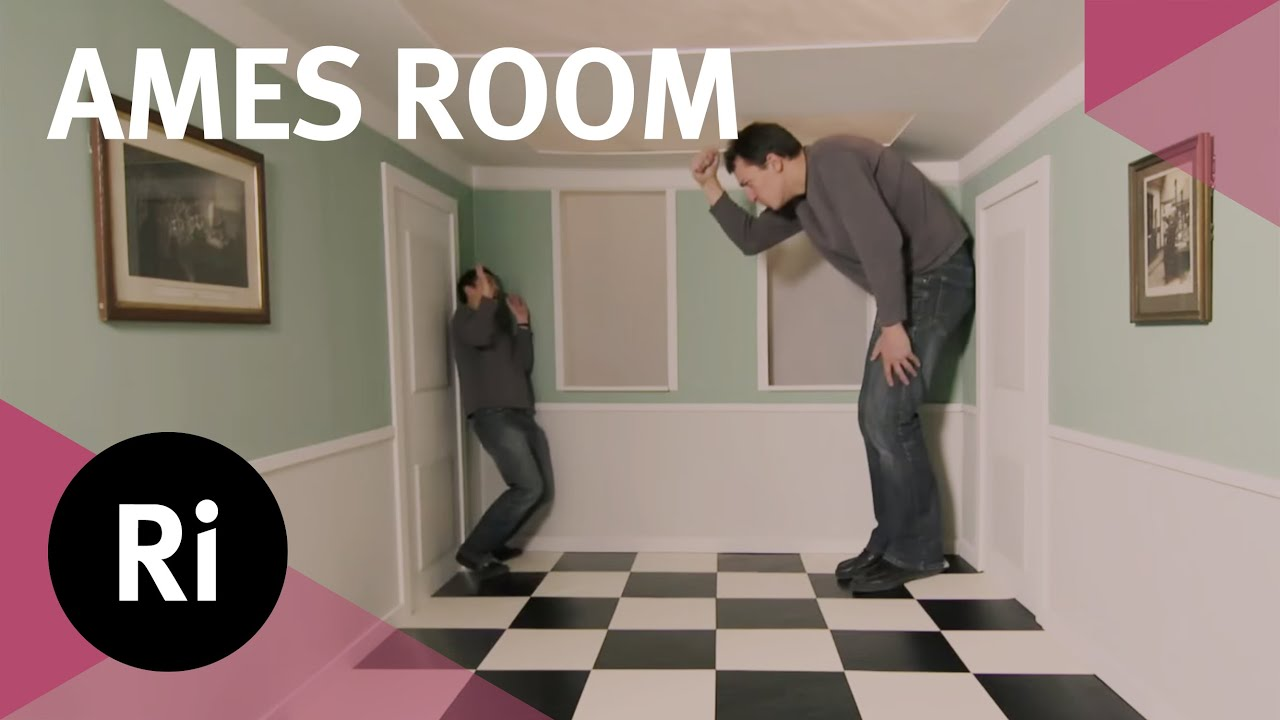
\includegraphics[width=3.5in,height=2.5in]{fiAmesRoom.jpg}

Perception is always influenced by by depth cues such as texture and
color that govern our perception of \(3D\) space. No matter how we try
to flatten it, the \(3D\) world is inescapable, says Wilkinson.

\hypertarget{graphing-space}{%
\section{13.3 Graphing space}\label{graphing-space}}

This section is about mapping an underlying mathematical space to a
\(2D\) or \(3D\) Euclidean space, which is where we see graphics. There
are four possibilities for the underlying space that Wilkinson
considers. These four are a connected space, a discrete space, a graph
(in the graph-theoretic sense), and a collection of nested spaces.

\hypertarget{mapping-connected-space-to-euclidean-space}{%
\subsection{13.3.1 Mapping connected space to Euclidean
space}\label{mapping-connected-space-to-euclidean-space}}

An example of mapping a non-Euclidean connected space to a connected
space is given as the conversion of a table of city block distances
between Manhattan landmarks and a \(2D\) map of those landmarks. This is
a felicitous example because of the way city blocks are laid out in
mid-Manhattan as a grid (except for Broadway and Central Park). An
interesting illusion occurs when we look at the geodesics in this
example. A zigzag pattern appears to be shorter than a straighter path
of equal length.

\hypertarget{mapping-affine-space-to-euclidean-space}{%
\subsection{13.3.1.2 Mapping affine space to Euclidean
space}\label{mapping-affine-space-to-euclidean-space}}

Euclidean space is isotropic (from a Greek word meaning \emph{the same
in any direction}). An affine transformation of Euclidean space results
in an anisotropic space. We can modify the formula for Euclidean
distance by adding a weight, \(w\), that differs in each direction
\(i\).

\[
d(x_j,x_k)=\left(\sum_{i=1}^n w_i ( x_{ij}-x_{ik})^2\right)^{1/2}
\]

This stretches or shrinks each dimension separately. An application of
this principle is Mahalanobis distance, which can give us a rotated
ellipse instead of a circle of distances as shown in textbook Figure
13.16.

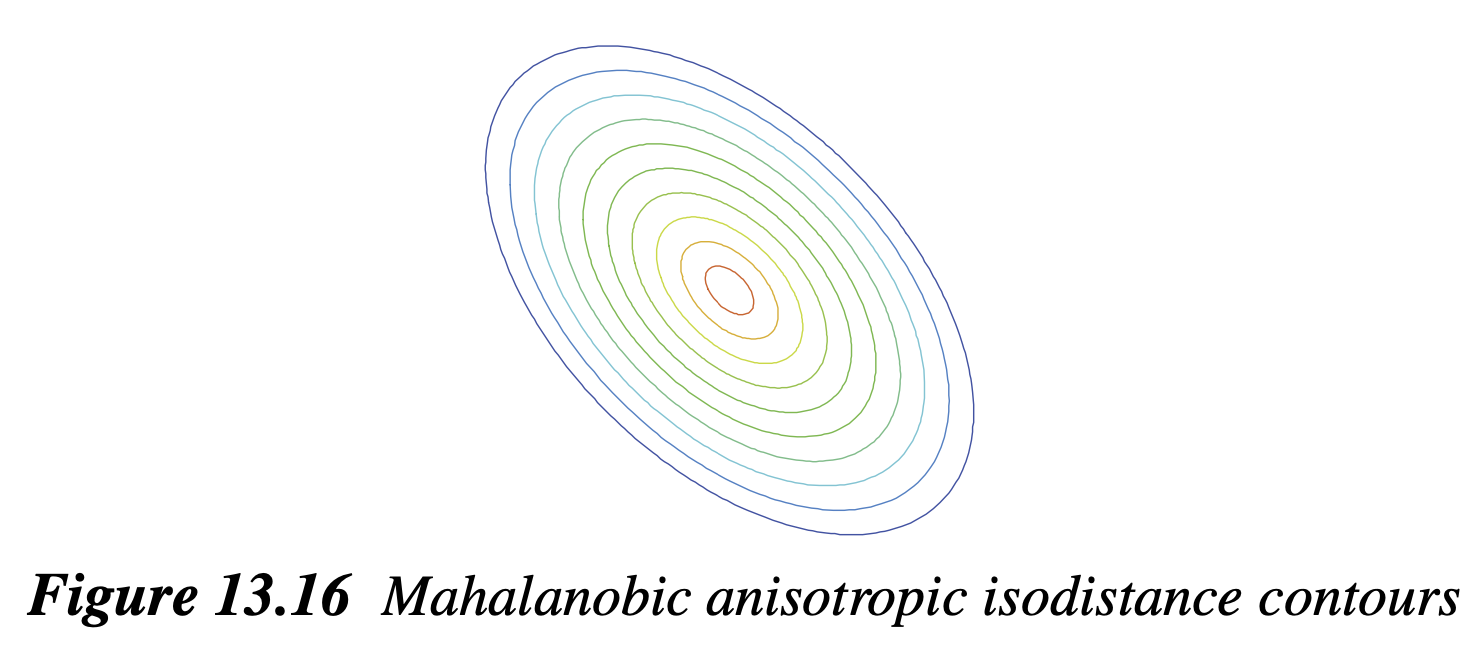
\includegraphics[width=3.5in,height=1.75in]{fiMahalanobis.png}

An example of this with the famous iris dataset is shown in textbook
Figure 13.17, where we see two species of iris, Versicolor and
Virginica. In the left panel, the star represents a new iris that we
would like to classify. At a glance it appears to belong to the red
ellipse, Versicolor. But extending the contours in the right panel shows
that it is slightly more like to belong to the blue ellipse, Virginica.
Thus if we're trying to evaluate anisotropic distances, we may need
multiple contours.

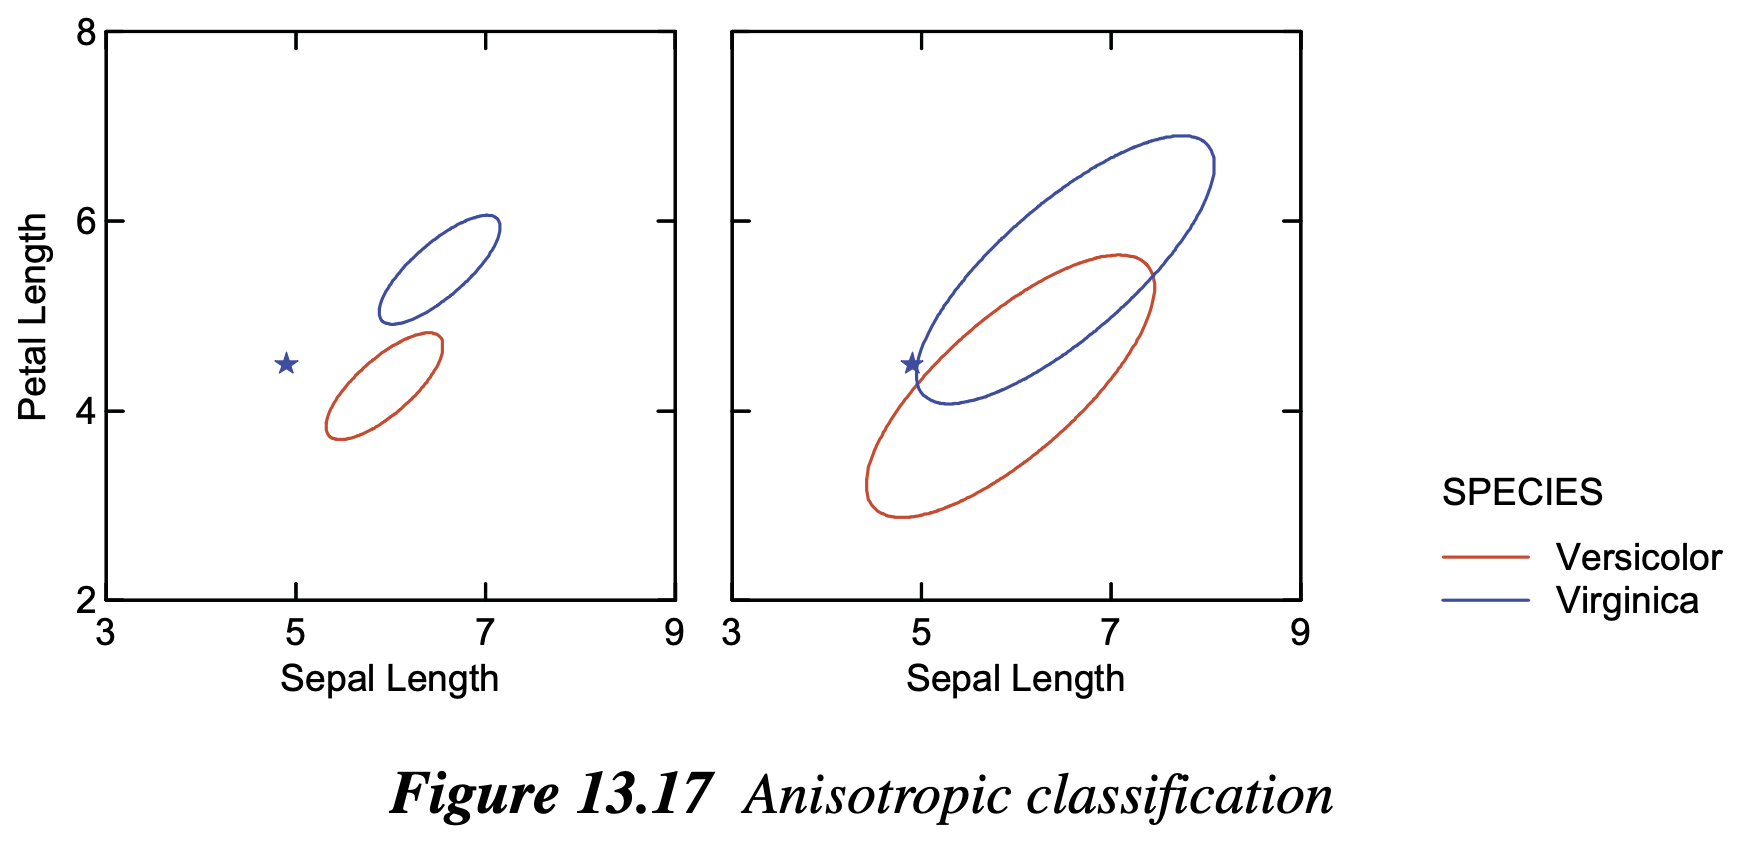
\includegraphics[width=4in,height=2in]{fiIris.png}

\hypertarget{sharing-space}{%
\subsection{13.3.1.4 Sharing space}\label{sharing-space}}

Symbols on scatterplots may represent points, but they have a nonzero
size. They occupy real space and often overlap as we saw in the Tableau
tutorial when we created a bubble plot of markets and reduced the
opacity of the symbols so they could be seen through each other.
Wilkinson returns to the beadlet anemones to show an example of a bubble
plot but in this case there is no sharing or stealing of space since the
size of the bubbles represents the size of the anemones. This is
atypical of bubble plots.

\hypertarget{label-layouts}{%
\subsection{13.3.1.5 Label layouts}\label{label-layouts}}

Graphics programs use algorithms called force-directed graph layouts to
move labels into positions such that they don't occlude each other. You
don't need to know much about these algorithms except that one might
work better than another in a given situation and some graphics software
lets you choose algorithms.

\hypertarget{mapping-discrete-space-to-euclidean-space}{%
\subsection{13.3.2 Mapping discrete space to Euclidean
space}\label{mapping-discrete-space-to-euclidean-space}}

When we map discrete space to Euclidean space, there are areas inside
the frame but outside the image of the mapping. That is, there is free
space where no points go. We may use free space for shape and size
aesthetics and for annotation.

Wilkinson provides a really good example of this in textbook Figure
13.22, where the middle row shows some egregious graphical practice and
the bottom row has been arranged to make the relationships more
perceivable. Note that both the ordering and spacing differs on the
bottom row.

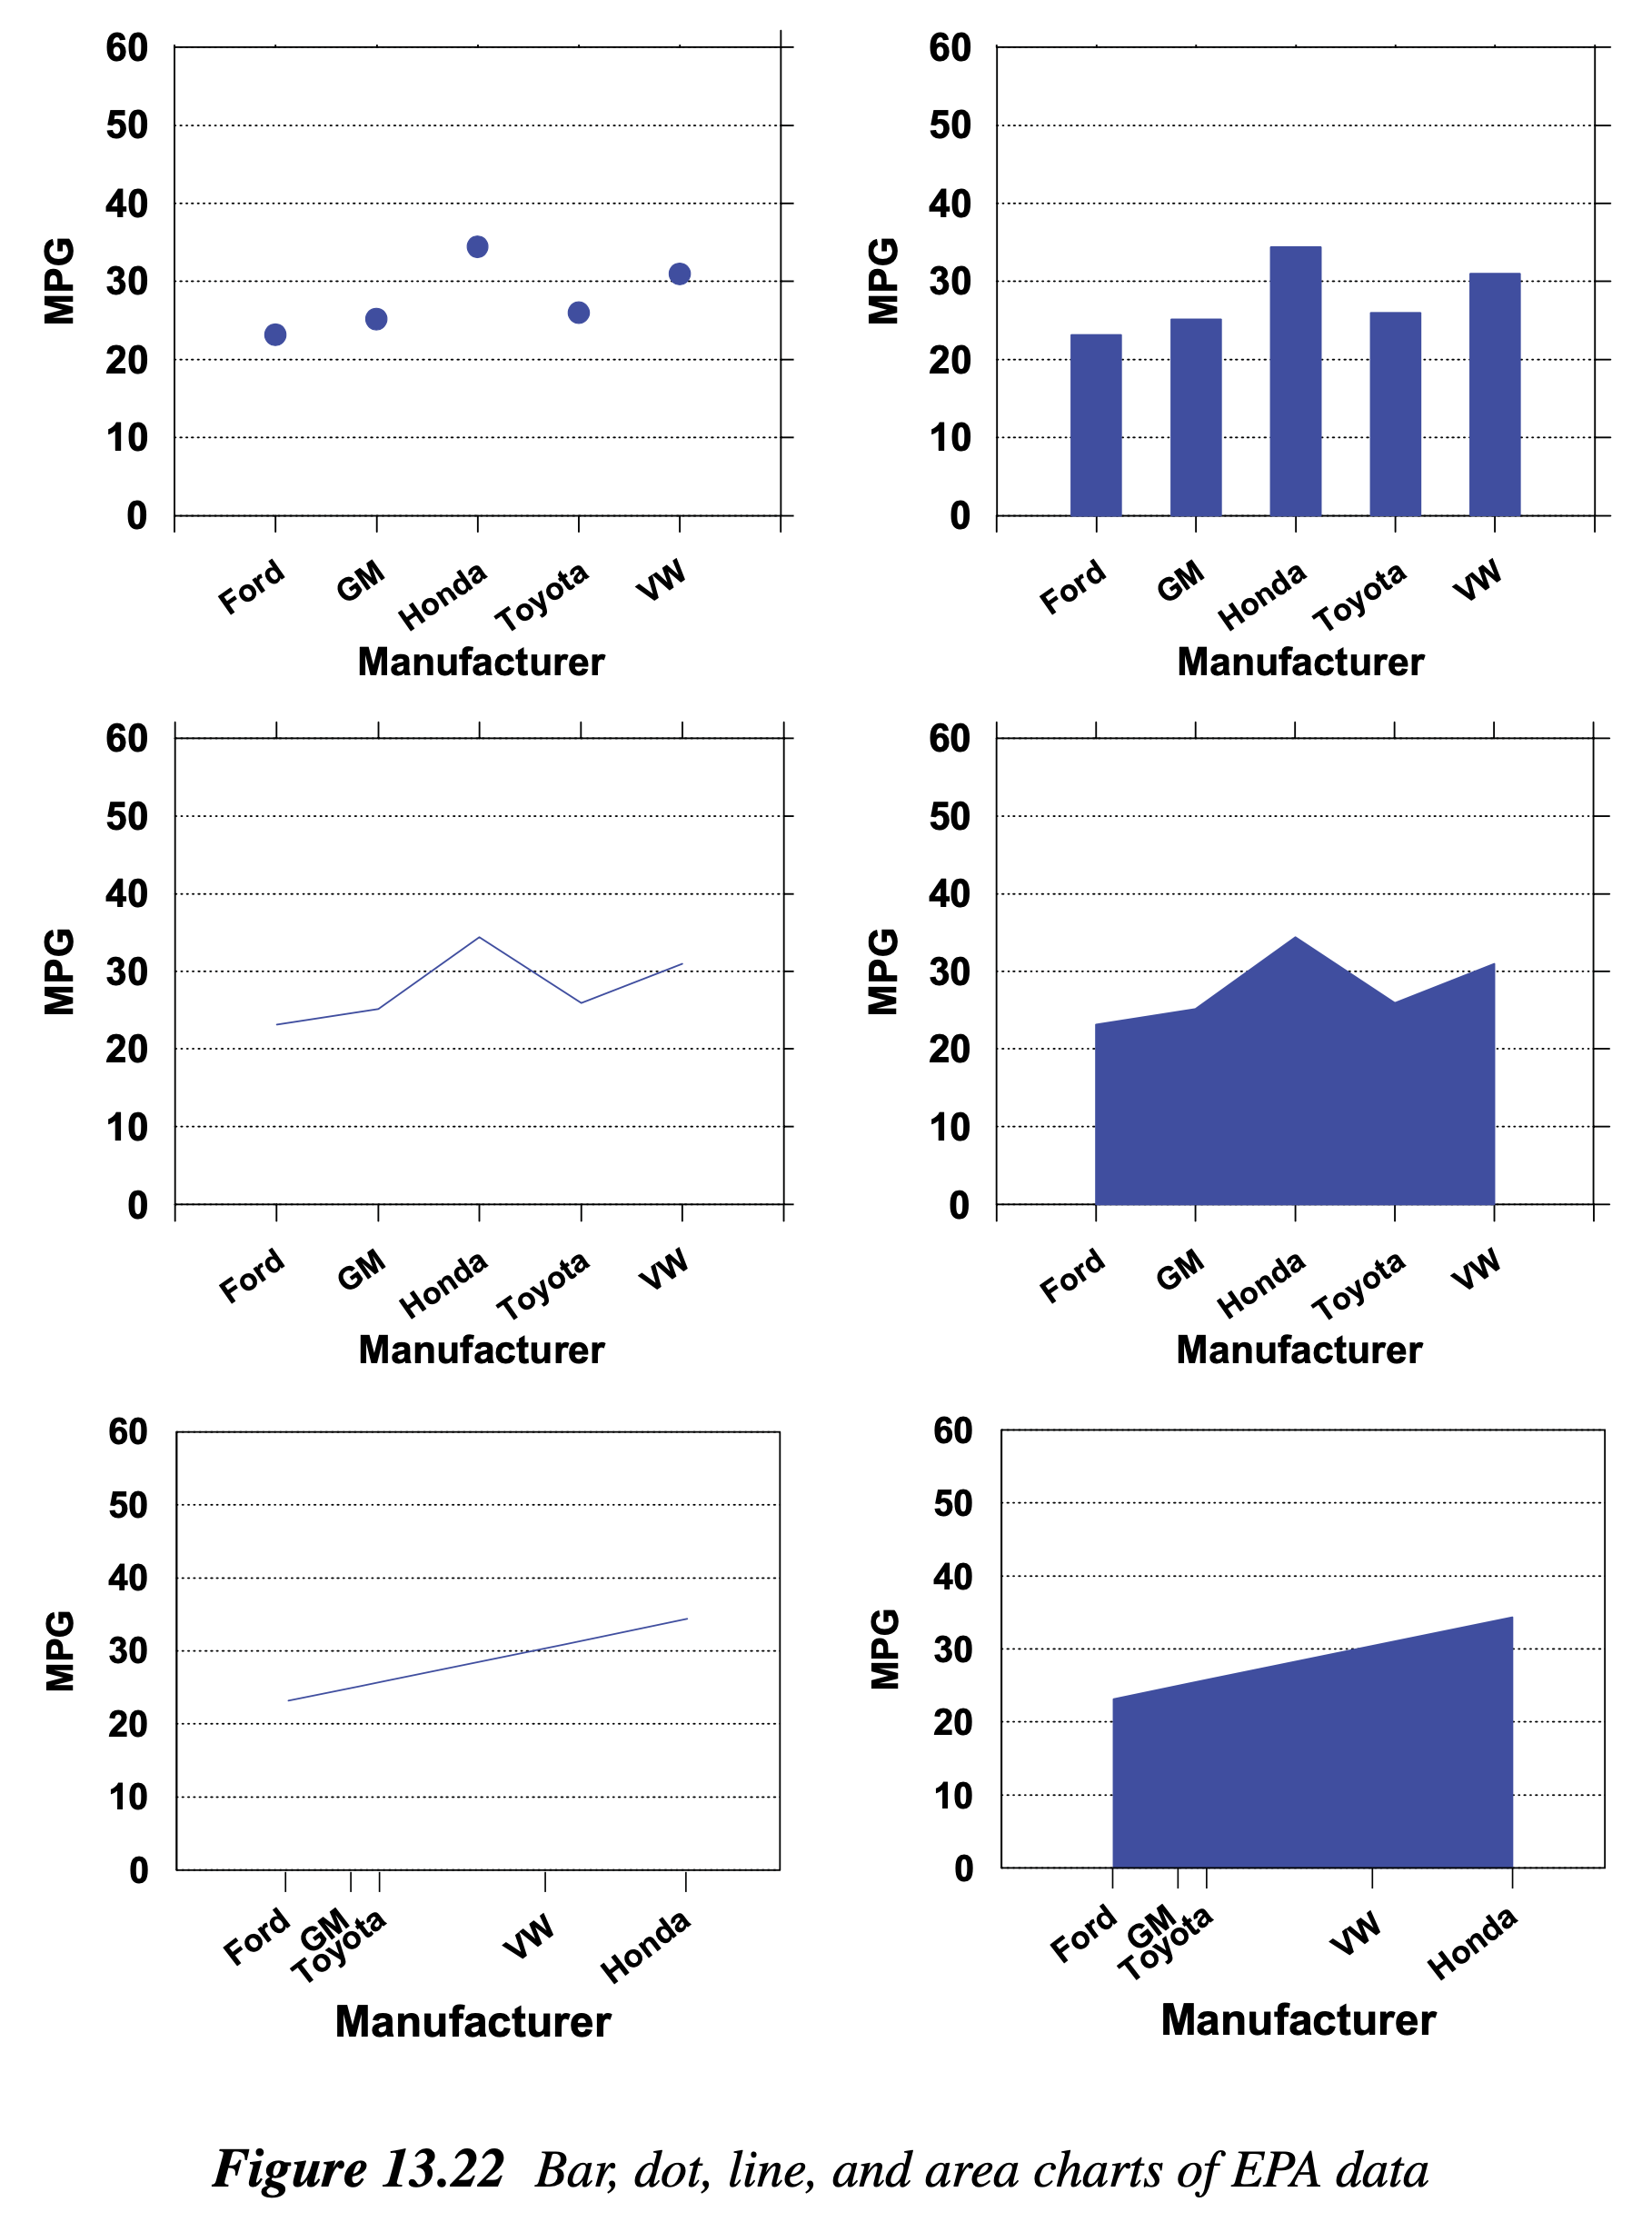
\includegraphics{fiEPAdata.png}

\hypertarget{mapping-graph-theoretic-space-to-euclidean-space}{%
\subsection{13.3.3 Mapping graph-theoretic space to Euclidean
space}\label{mapping-graph-theoretic-space-to-euclidean-space}}

Wilkinson covers spanning trees (including the minimum spanning tree
mentioned earlier), ultrametric trees, and additive trees in this
subsection. Of special note are dendrograms, which result from
clustering algorithms. A number of dendrograms are depicted, although
Wilkinson never calls them by name.

An ultrametric space is not explicitly defined by Wilkinson, but
Wikipedia provides a concise definition where instead of the triangle
inequality:

\[
d(x,z) \leqslant d(x,y)+d(y,z)
\]

\noindent distances in the space obey the ultrametric inequality:

\[
d(x,z) \leqslant \max \left\{d(x,y),d(y,z)\right\}
\]

A dendrogram is an ultrametric tree. Wilkinson shows three dendrograms
in Figure 13.26, each constructed using a different algorithm on the
anemone data. In this case, average linkage works best to reveal the
true clusters, but in practice, no one method (single, linkage, complete
linkage, or average linkage) dominates all cases. Thus, for
visualization purposes, it is often best to try all three. Software that
creates dendrograms, such as several R packages, usually allows you to
select the linkage algorithm.

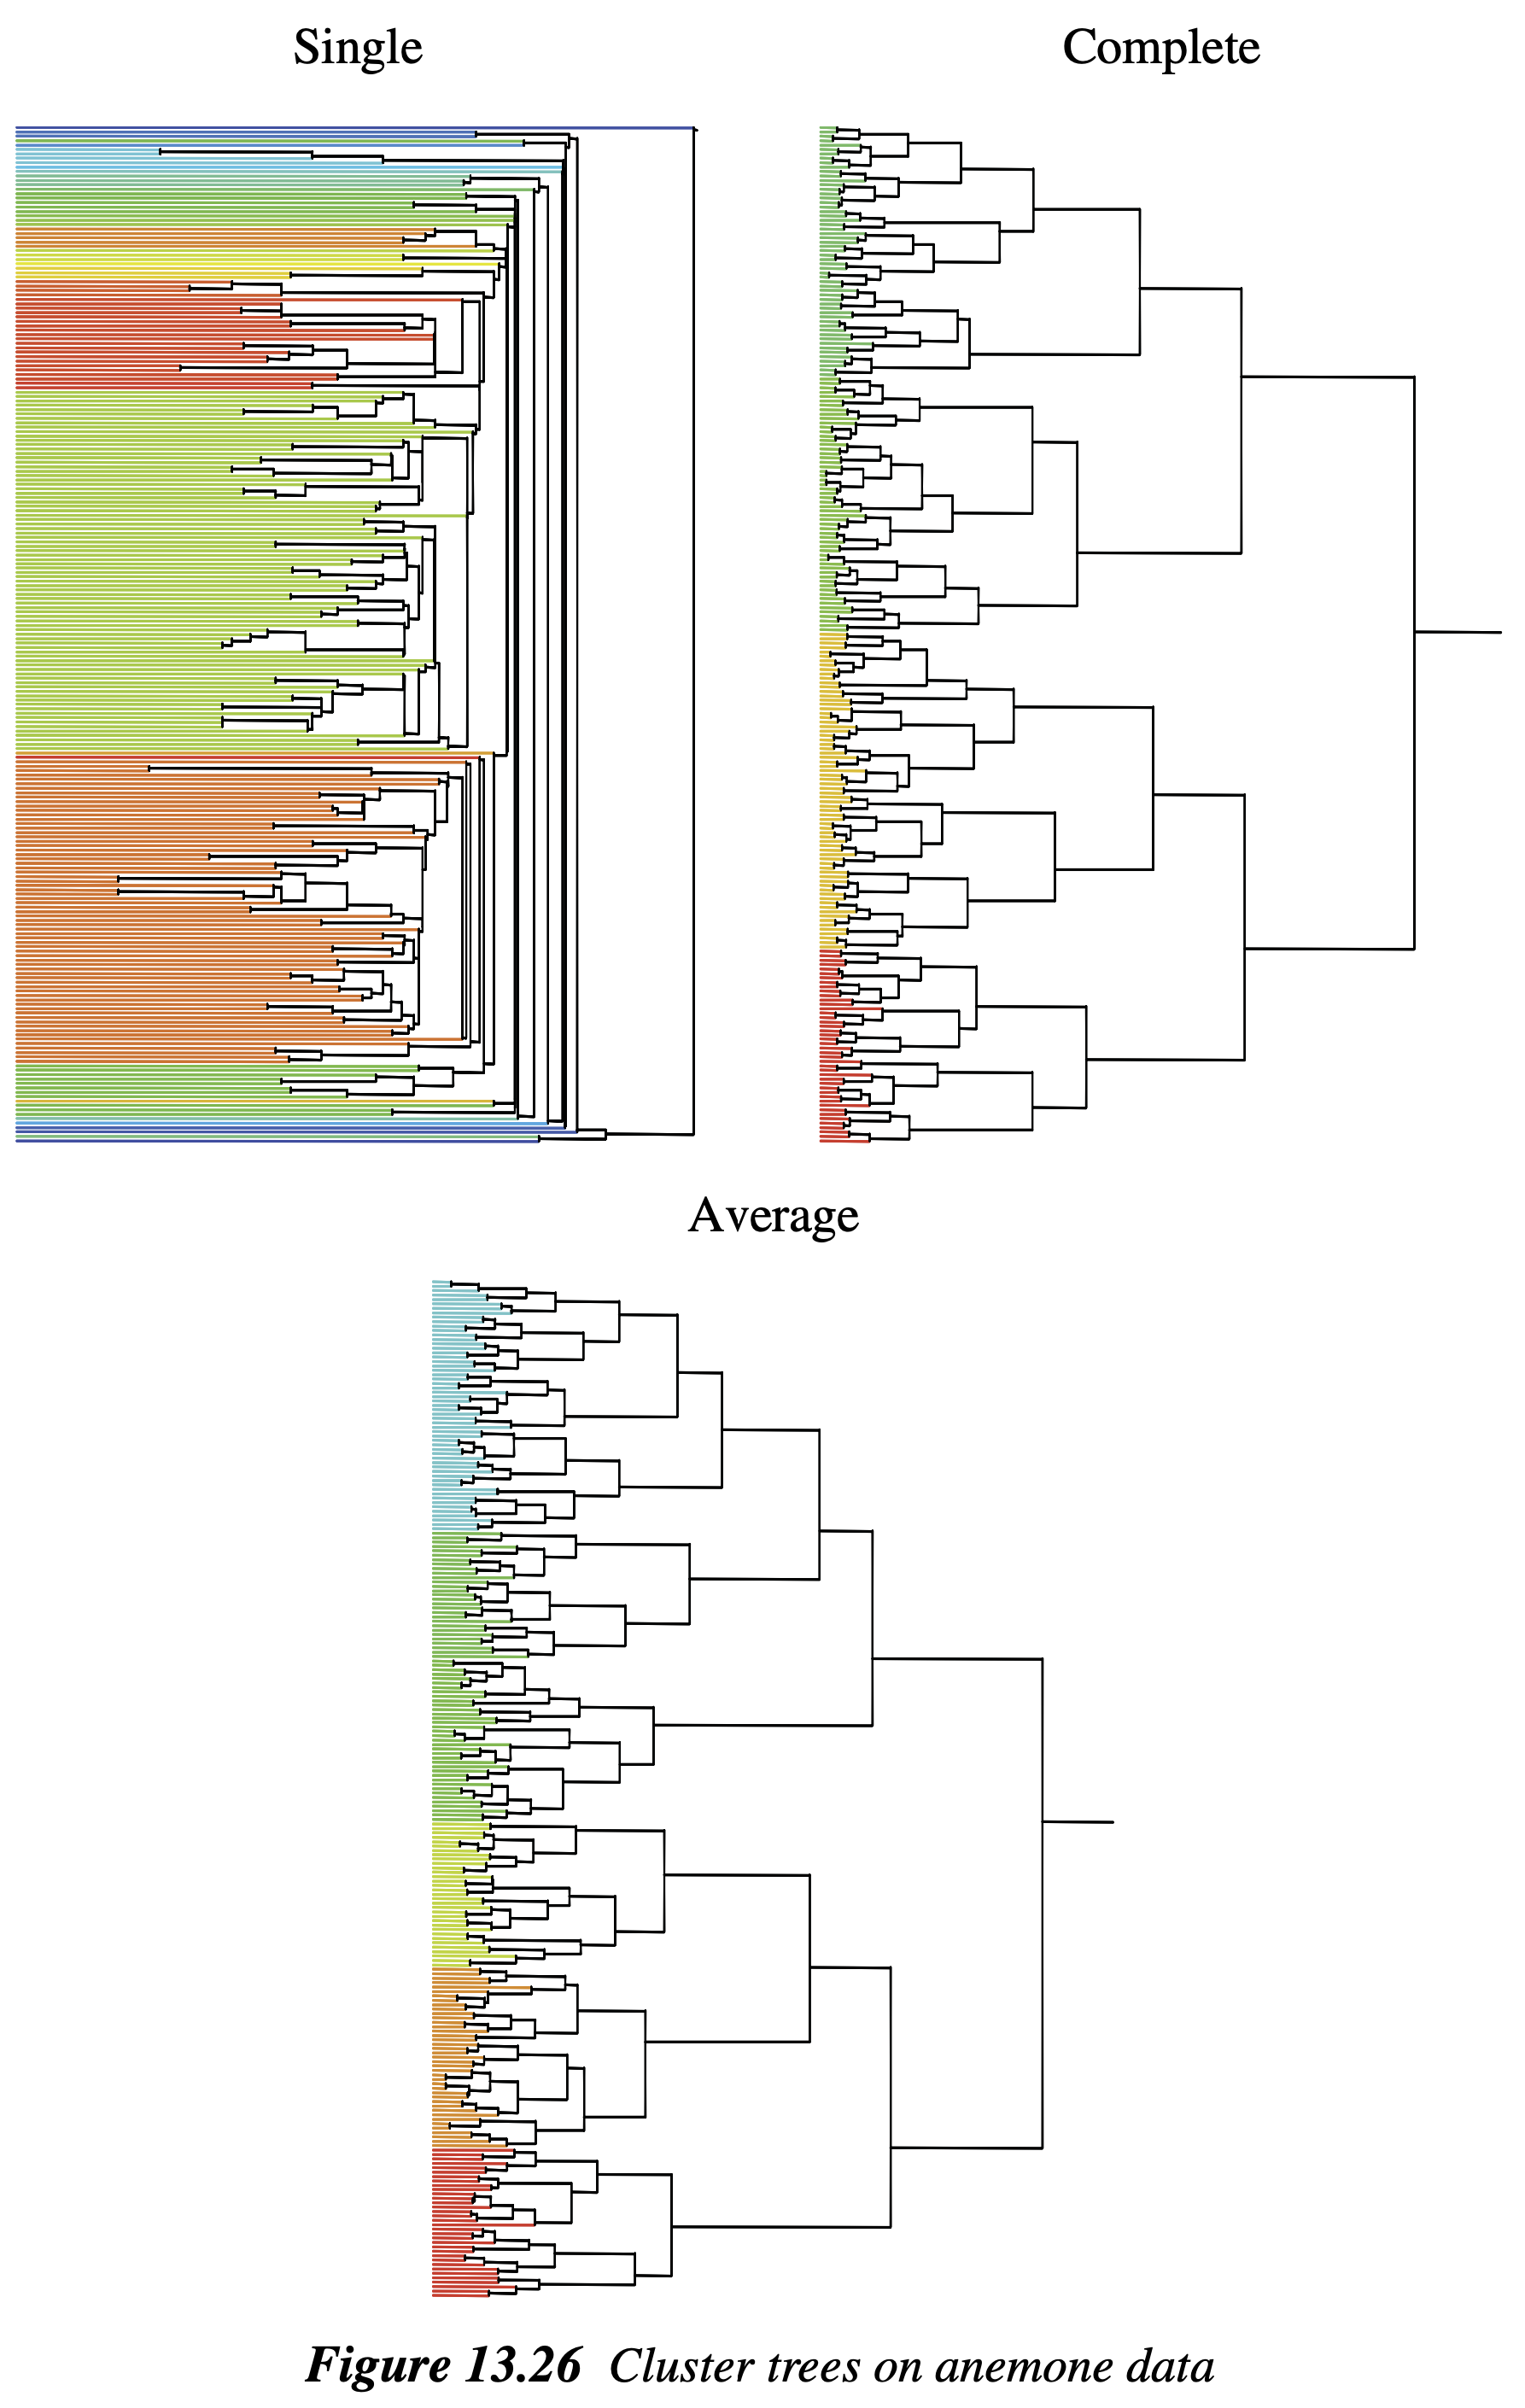
\includegraphics[height=3.5in,width=2.5in]{fiDendrograms.png}

\hypertarget{mapping-nested-space-to-euclidean-space}{%
\subsection{13.3.4 Mapping nested space to Euclidean
space}\label{mapping-nested-space-to-euclidean-space}}

Wilk-inson describes treemaps, Temple MVV, and region trees in this
subsection. All of these represent nested spaces in Euclidean spaces,
but some are more successful than others. For example, treemaps have
been popular in showing the contents of disk-based filesystems.

The procedure for constructing a treemap is given in this subsection,
but it is usual for software to carry out the procedure, with the user
simply specifying the variables to be used and a linkage algorithm.
Textbook Figure 13.30 shows an example of a tree converted to a treemap,
but more information is needed than is shown in the picture to
understand how it is done. First there is some variable for splitting
the tree, then there is some variable for determining the size of each
tile.

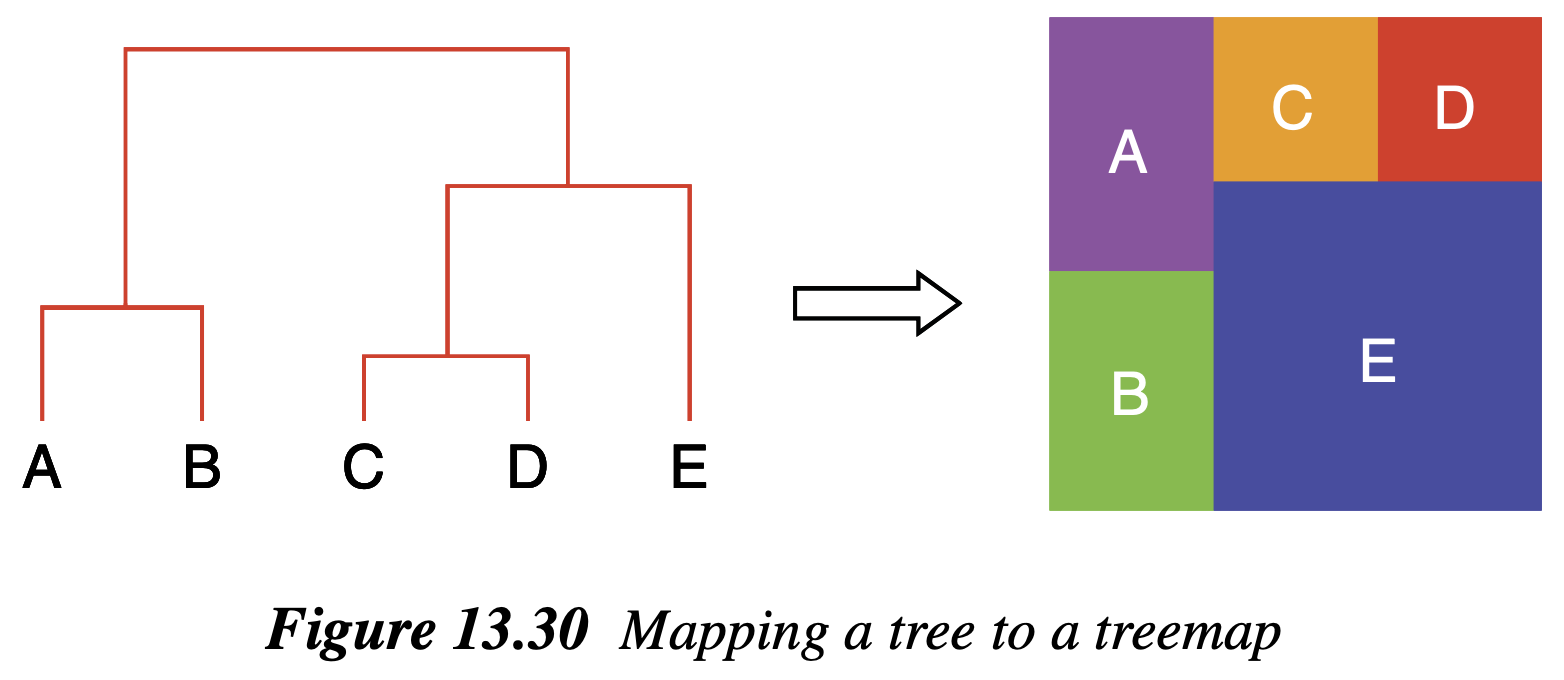
\includegraphics[height=1.5in,width=4in]{fiTreeToTreemap.png}

To make this process clearer, consider the following treemap from Butler
Analytics. The tiles are sized according to number of voters and the
tiles are created by a two-level hierarchy of state and county. Notice
that the tiles are colored by political affiliation.

\bigskip

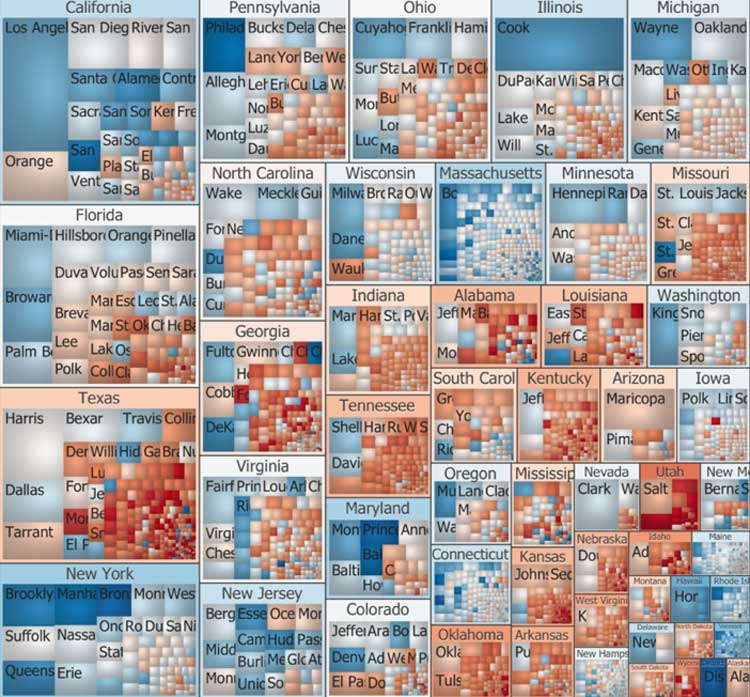
\includegraphics{fiVotingTreemap.jpg}

Wilkinson strongly prefers region trees over Temple MVV and has much
negative to say about OLAP (online analytical processing) cubes, which
are the basis for Temple MVV. As an example, he shows two views of the
Titanic data, with textbook Figure 13.33 supplying the Temple MVV view
and textbook Figure 13.34 supplying the region tree view.

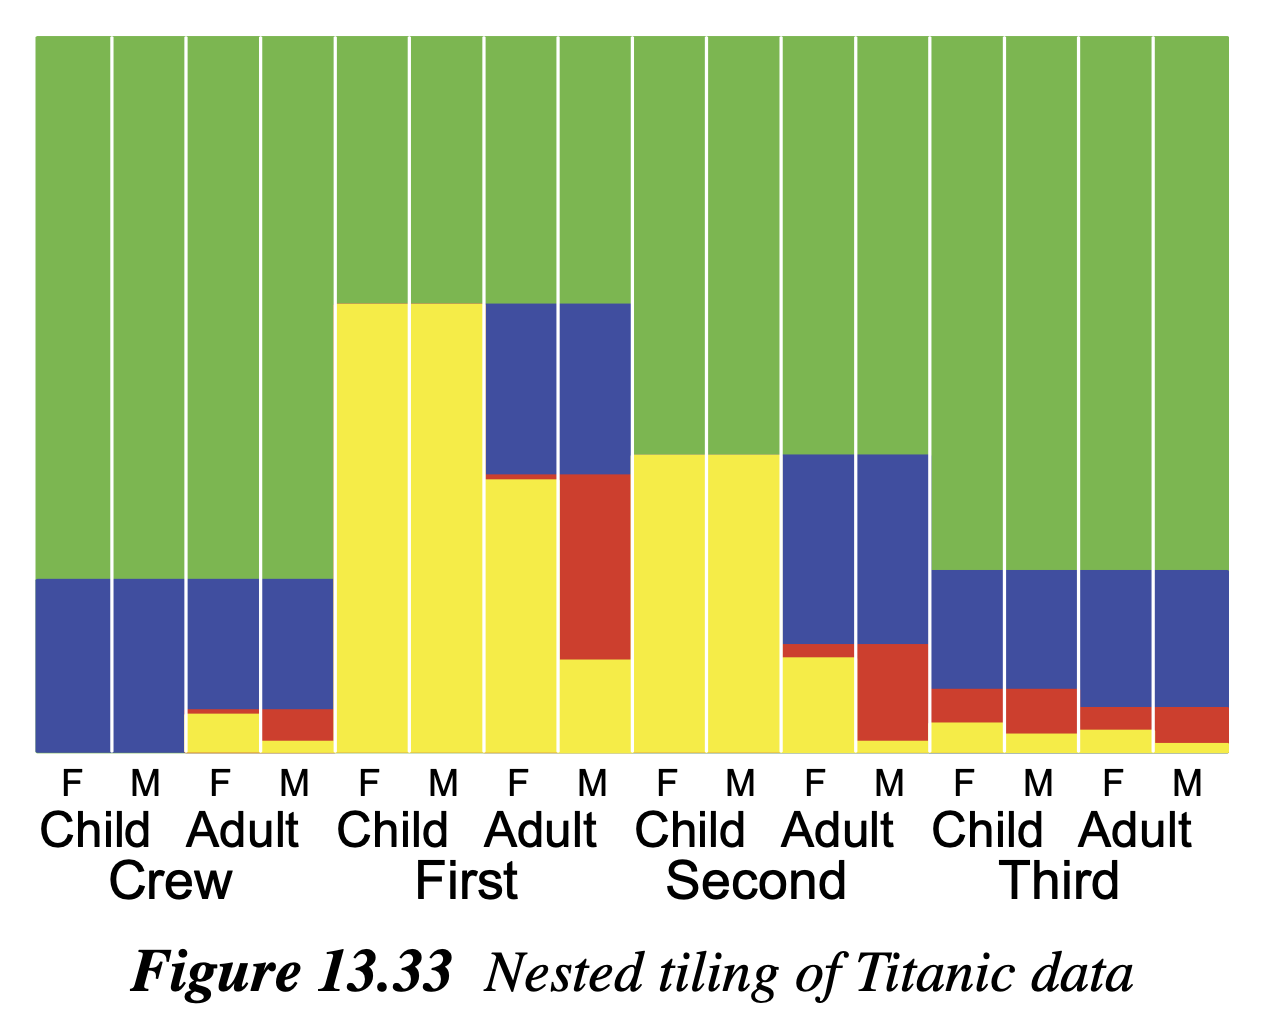
\includegraphics{fiTitanicTempleMVV.png}

This famous dataset lists the survivors of the Titanic, according to
age, class, and gender. As you may know, the children and most of the
women in first class survived, but the other groups suffered more
fatalities according to class and gender. This is fairly easy to see in
the region tree but much harder in the Temple MVV visualization.

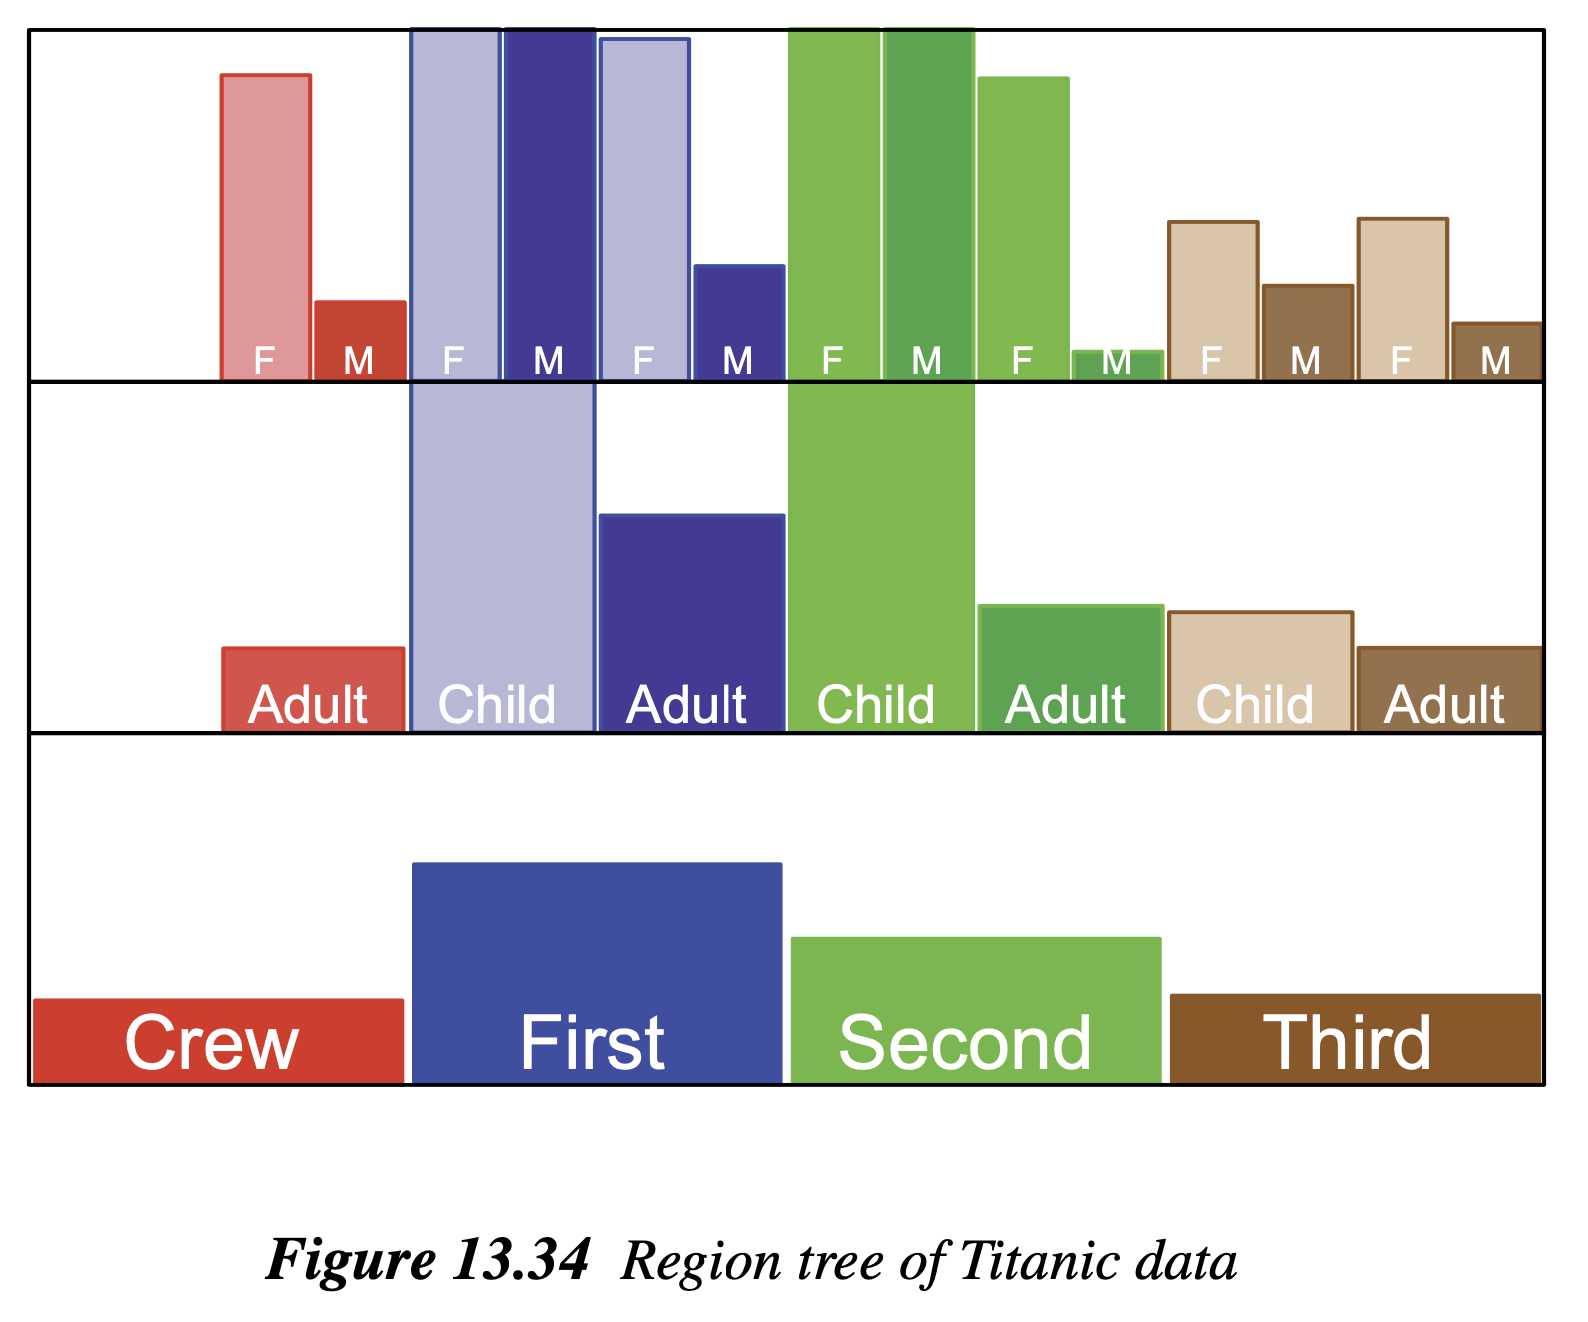
\includegraphics{fiTitanicRegionTree.png}

The region tree exemplifies a faceted display, a very popular data
visualization tool for dividing data into facets of interest. In this
case we see three separate facets, gender at the top, age in the middle,
and class at the bottom.

\hypertarget{conclusion}{%
\section{Conclusion}\label{conclusion}}

These notes just gloss over some of the important points of Wilkinson's
chapter on space. It is worthwhile to read the chapter for more detail
and for references to some of the relevant literature on the topic.
Although the book was published in 2005, most of the material is
relevant today and it is possible to update your knowledge of the other
areas by following the citation networks of the references. The only
deficiency is that he spells Shneiderman wrong, making it a little
harder to search for information about treemaps, of which there are many
varieties today.
